\documentclass[]{book}
\usepackage{lmodern}
\usepackage{amssymb,amsmath}
\usepackage{ifxetex,ifluatex}
\usepackage{fixltx2e} % provides \textsubscript
\ifnum 0\ifxetex 1\fi\ifluatex 1\fi=0 % if pdftex
  \usepackage[T1]{fontenc}
  \usepackage[utf8]{inputenc}
\else % if luatex or xelatex
  \ifxetex
    \usepackage{mathspec}
  \else
    \usepackage{fontspec}
  \fi
  \defaultfontfeatures{Ligatures=TeX,Scale=MatchLowercase}
\fi
% use upquote if available, for straight quotes in verbatim environments
\IfFileExists{upquote.sty}{\usepackage{upquote}}{}
% use microtype if available
\IfFileExists{microtype.sty}{%
\usepackage{microtype}
\UseMicrotypeSet[protrusion]{basicmath} % disable protrusion for tt fonts
}{}
\usepackage[margin=1in]{geometry}
\usepackage{hyperref}
\hypersetup{unicode=true,
            pdftitle={It Can Be Shown},
            pdfauthor={Benjamin Nutter},
            pdfborder={0 0 0},
            breaklinks=true}
\urlstyle{same}  % don't use monospace font for urls
\usepackage{longtable,booktabs}
\usepackage{graphicx,grffile}
\makeatletter
\def\maxwidth{\ifdim\Gin@nat@width>\linewidth\linewidth\else\Gin@nat@width\fi}
\def\maxheight{\ifdim\Gin@nat@height>\textheight\textheight\else\Gin@nat@height\fi}
\makeatother
% Scale images if necessary, so that they will not overflow the page
% margins by default, and it is still possible to overwrite the defaults
% using explicit options in \includegraphics[width, height, ...]{}
\setkeys{Gin}{width=\maxwidth,height=\maxheight,keepaspectratio}
\IfFileExists{parskip.sty}{%
\usepackage{parskip}
}{% else
\setlength{\parindent}{0pt}
\setlength{\parskip}{6pt plus 2pt minus 1pt}
}
\setlength{\emergencystretch}{3em}  % prevent overfull lines
\providecommand{\tightlist}{%
  \setlength{\itemsep}{0pt}\setlength{\parskip}{0pt}}
\setcounter{secnumdepth}{5}
% Redefines (sub)paragraphs to behave more like sections
\ifx\paragraph\undefined\else
\let\oldparagraph\paragraph
\renewcommand{\paragraph}[1]{\oldparagraph{#1}\mbox{}}
\fi
\ifx\subparagraph\undefined\else
\let\oldsubparagraph\subparagraph
\renewcommand{\subparagraph}[1]{\oldsubparagraph{#1}\mbox{}}
\fi

%%% Use protect on footnotes to avoid problems with footnotes in titles
\let\rmarkdownfootnote\footnote%
\def\footnote{\protect\rmarkdownfootnote}

%%% Change title format to be more compact
\usepackage{titling}

% Create subtitle command for use in maketitle
\newcommand{\subtitle}[1]{
  \posttitle{
    \begin{center}\large#1\end{center}
    }
}

\setlength{\droptitle}{-2em}
  \title{It Can Be Shown}
  \pretitle{\vspace{\droptitle}\centering\huge}
  \posttitle{\par}
\subtitle{Notes on Statistical Theory}
  \author{Benjamin Nutter}
  \preauthor{\centering\large\emph}
  \postauthor{\par}
  \predate{\centering\large\emph}
  \postdate{\par}
  \date{2016-08-10}

\usepackage{amssymb} 
\usepackage{arydshln} 
\usepackage{caption} 
\usepackage{graphicx} 
\usepackage{hhline} 
\usepackage{longtable} 
\usepackage{multirow} 
\usepackage[dvipsnames,table]{xcolor} 
\makeatletter 
\newcommand*\vdashline{\rotatebox[origin=c]{90}{\$\dabar@\dabar@\dabar@\$}} 
\makeatother

\begin{document}
\maketitle

{
\setcounter{tocdepth}{1}
\tableofcontents
}
\chapter{Introduction}\label{introduction}

There is one phrase that makes me cringe every time I see it. It's a
phrase that embodies feelings of frustration, inadequacy, and failure to
understand. That phrase:

\begin{quote}
It can be shown
\end{quote}

Everytime I read that phrase, I would look at the subsequent result and
think ``Really? It can?''

This book is a collection of notes that I've put together to avoid
having to feel that way in the future. It is, essentially, a collection
of definitions and proofs that have helped me understand and apply
mathematical and statistical theory. Most imporantly, it spells even the
smallest steps along each development so that I don't have to worry
about solving it again in the future.

You won't find much in the way of application. There are no exercises.
There is only minimal explanation. My intent is to show development of
statistical theory and nothing else.

\chapter{Bernoulli Distribution}\label{bernoulli-distribution}

\section{Probability Mass Function}\label{probability-mass-function}

A random variable is said to have a Bernoulli Distribution with
parameter \(p\) if its probability mass function is: \[p(x)=\left\{ 
        \begin{array}{ll}
            p^x(1-p)^{1-x}, & x=0,1\\
            0       & \mathrm{otherwise}
        \end{array} 
    \right. \] Where \(p\) is the probability of a success.

\section{Cumulative Mass Function}\label{cumulative-mass-function}

\label{Bernoulli1} \[P(x)=\left\{
        \begin{array}{lll}
            0   & x<0\\
            1-p & x=0\\
            1   & 1\leq x
        \end{array}
    \right. \]

\begin{figure}[htbp]
\centering
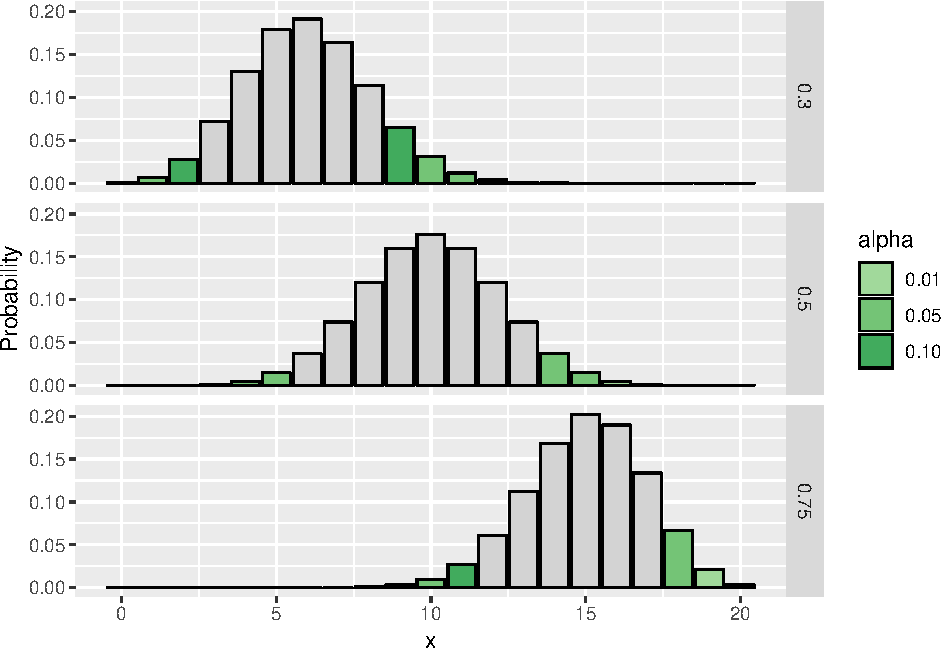
\includegraphics{_main_files/figure-latex/unnamed-chunk-2-1.pdf}
\caption{\label{fig:unnamed-chunk-2}The graphs on the left and right show a
Binomial Probability Distribution and Cumulative Distribution Function,
respectively, with \(p=.4\). Note that this is identical to a Binomial
Distribution with parameters \(n=1\) and \(p=.4\).}
\end{figure}

\section{Expected Values}\label{expected-values}

\[ 
\begin{align*}
E(X) 
  &= \sum\limits_{i=0}^{1} x\cdot p(x) \\
    &= \sum\limits_{i=0}^{1} x \cdot p^{x} (1-p)^{1-x}\\
  &= 0 \cdot p^{0} (1-p)^{1-0} + 1 \cdot p^{1} (1-p)^{1-1}\\
  &= 0 + p (1-p)^{0}\\
    &= p\\
    \\
    \\
E(X^{2}) 
  &= \sum\limits_{i=0}^{1} x^2 \cdot p(x)\\
  &= \sum\limits_{i=0}^{1} x^{2} \cdot p^x (1-p)^{1-x}\\
  &= \sum\limits_{i=0}^{1} 0^{2} \cdot p^0 (1-p)^{1-0} + 1^2 \cdot p^1 (1-p)^{1-1}\\
  &= 0 \cdot 1 \cdot 1 + 1 \cdot p \cdot 1 \\
    &= 0 + p\\
    &= p\\
    \\
    \\
\mu &= E(X) = p\\
  \\
  \\
\sigma^2 
  &= E(X^2) - E(X)^2 \\
  &= p-p^2 \\
  &= p(1-p)
\end{align*}
\]

\section{Moment Generating Function}\label{moment-generating-function}

\[\begin{align*}
M_{X}(t)
    &= E(e^{tX}) \\
    &= \sum\limits_{i=0}^{1} e^{tx} p(x) \\
    &= \sum\limits_{i=0}^{1} e^{tx} p^{x} (1-p)^{1-x}\\
    &= e^{t0} p^0 (1-p)^{1-0} + e^t p^t (1-p)^{1-1}\\
    &= (1-p) + e^t p\\
    &=pe^t + (1-p) \\
    \\
    \\
M^{(1)}_X(t) &= pe^t\\
  \\
  \\
M^{(2)}_X(t) &= pe^t\\
  \\
  \\
E(X)
    &=M^{(1)}_X(0)\\
    &= pe^0\\
    &= pe^0\\
    &= p\\
    \\
    \\
E(X^2)
    &= M^{(2)}_X(0)\\
    &= pe^0\\
    &= p\\
    \\
    \\
\mu
  &= E(X)\\
    &= p\\
  \\
  \\
\sigma^2
    &= E(X^2) - E(X)^2 \\
    &= p - p^2 \\
    &= p (1-p)
\end{align*}
\]

\section{Theorems for the Bernoulli
Distribution}\label{theorems-for-the-bernoulli-distribution}

\subsection{Validity of the
Distribution}\label{validity-of-the-distribution}

\[\sum\limits_{x=0}^{1}p^x(1-p)^{1-x}=1\]

\emph{Proof:}

\[\begin{align*}
\sum\limits_{x=0}^{1} p^x (1-p)^{1-x}
    &= p^0 (1-p)^1 + p^1 (1-p)^0 \\
    &= (1-p) + p \\
    &= 1
\end{align*}\]

\subsection{Sum of Bernoulli Random
Variables}\label{sum-of-bernoulli-random-variables}

Let \(X_1,X_2,\ldots,X_n\) be independent and identically distributed
random variables from a Bernoulli distribution with parameter \(p\). Let
\(Y=\sum\limits_{i=1}^{n}X_i\).\textbackslash{} Then \(Y\sim\)
Binomial\((n,p)\)

\emph{Proof:} \[\begin{align*}
M_Y(t)
    &= E(e^{tY}) \\
    &= E(e^{tX_1} e^{tX_2} \cdots e^{tX_n}) \\
    &= E(e^{tX_1}) E(e^{tX_2}) \cdots E(e^{tX_n}) \\
  &= (pe^t+(1-p)) (pe^t+(1-p)) \cdots (pe^t+(1-p)) \\
    &= (pe^t+(1-p))^n
\end{align*}\]

Which is the moment generating function of a Binomial random variable
with parameters \(n\) and \(p\). Thus, \(Y\sim\) Binomial\((n,p)\).

\chapter{Binomial Distribution}\label{binomial-distribution}

\section{Probability Mass Function}\label{probability-mass-function-1}

A random variable is said to follow a Binomial distribution with
parameters \(n\) and \(p\) if its probability mass function is:

\[p(x)=
    \left\{
        \begin{array}{ll}
            {n \choose x} p^x (1-p)^{n-x},  & x=0,1,2,\ldots,n\\
            0               & \mathrm{otherwise}
        \end{array}
    \right. \]

Where \(n\) is the number of trials performed and \(p\) is the
probability of a success on each individual trial.

\section{Cumulative Mass Function}\label{cumulative-mass-function-1}

\[ P(x)=
    \left\{
        \begin{array} {lll}
            0                           & x<0\\
            \sum\limits_{i=0}^{x} {n \choose i} p^i (1-p)^{n-i}     & 0 \leq x=0,1,2,\ldots,n\\
            1                           & n\leq x
        \end{array}
    \right. \]

A recursive form of the cdf can be derived and has some usefulness in
computer applications. With it, one need only initiate the first value
and additional cumulative probabilities can be calculated. It is derived
as follows:

\[\begin{align*} 
F(x+1)
    &= {n\choose x+1} p^{x+1} (1-p)^{n-(x+1)} \\
    &= \frac{n!}{(x+1)!(n-(x+1))!} p^{x+1} (1-p)^{n-(x+1)} \\
  &= \frac{n!}{(x+1)!(n-x-1)!} p^{x+1} (1-p)^{n-x-1} \\
  &= \frac{(n-x)n!}{(x+1)x!(n-x)(n-x-1)!} p \cdot p^x \frac{(1-p)^{n-x}}{(1-p)} \\
  &= \frac{(n-x)n!}{(x+1)x!(n-x)!} \cdot \frac{p}{1-p} p^x (1-p)^{n-x} \\
  &= \frac{p}{1-p} \cdot \frac{n-x}{x+1} \cdot \frac{n!}{x!(n-x)!} p^x (1-p)^{n-x} \\
  &= \frac{p}{1-p} \cdot \frac{n-x}{x+1} \cdot {n\choose x} p^x (1-p)^{n-x} \\
    &= \frac{p}{1-p} \cdot \frac{n-x}{x+1} \cdot F(x)
\end{align*}\]

\begin{figure}[htbp]
\centering
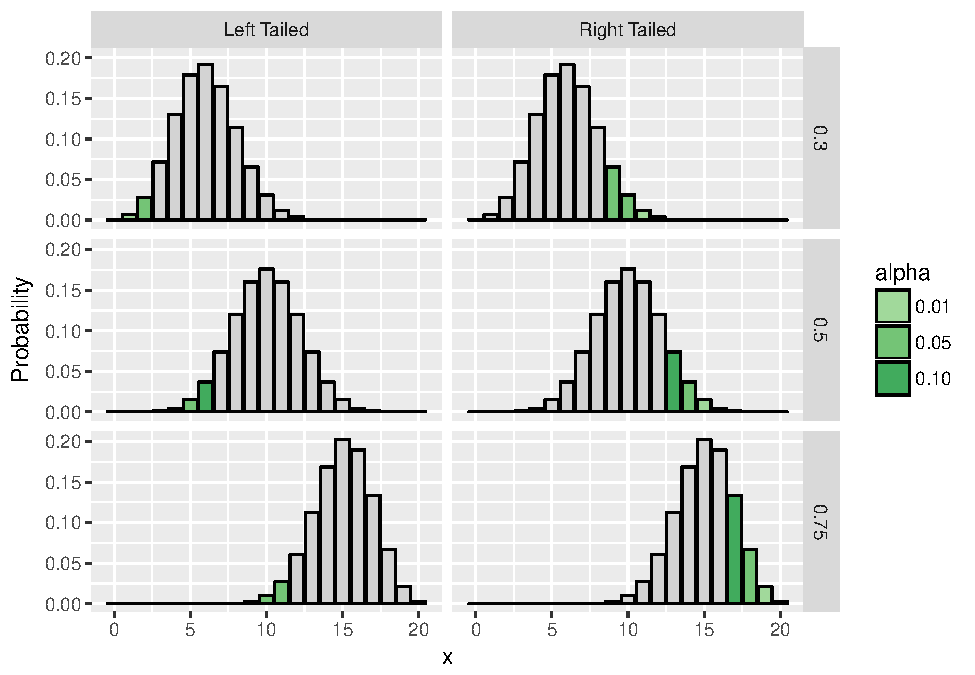
\includegraphics{_main_files/figure-latex/unnamed-chunk-3-1.pdf}
\caption{\label{fig:unnamed-chunk-3}The graphs on the left and right show a
Binomial Probability Distribution and Cumulative Distribution Function,
respectively, with \(n=10\) and \(p=.4\).}
\end{figure}


\end{document}
